
\chapter{Beyond Chat: Collaborative Editors Enhance Human Involvement and Agency When Co-Writing with Large Language Models} \label{c:tc5} 


\section{Link to thesis}

This chapter addresses my core research question by focusing on interfaces that preserve \textbf{human creative agency}, examining \textbf{how interaction design shapes the roles of humans and AI in co-creative processes}, and informing \textbf{interaction design principles for effective human-AI co-creation}.

In a previous chapter, I conducted an initial exploration of dialogic interaction by adapting a text-completion language model into a conversational co-writer. There, I argued that effective dialogic co-creativity involves more than a simple two-way conversation; it requires interaction both \textit{through} and \textit{about} the creative product.

Between that early 2022 work and the paper presented in this chapter (conducted in 2024 and published in 2025) there was significant progress in generative language models. Indeed, interaction converged to conversational interfaces as the dominant paradigm. While these interfaces can facilitate dialogue to align understanding, I argue they predominantly support interaction \textit{about} the creative product, rather than \textit{through} it, simply because they lack the space to do so.

I hypothesised that an interface providing such a collaborative space could better support these two interaction modes. The research presented in this chapter tested this hypothesis through the iterative development of functional co-creative system prototypes in two versions, Vorges and Common AI. These systems combined a chat interface with a collaborative text editor, allowing the user and the AI to converse and edit a stateful piece of writing in separate but integrated spaces.

These prototypes were evaluated through two user studies, which provided empirical qualitative and quantitative evidence addressing my research questions.

Firstly, my \textbf{core research question} centres on designing generative AI interactions that effectively maintain human agency. Results demonstrated that chat-only interfaces restricted user agency and involvement at the writing level. In contrast, the hybrid interface, which combined a conversational and  a collaborative writing space, resulted in users reporting higher levels of agency and active involvement in the co-creative writing process.

Secondly, my research subquestion number one (R1) examines how interaction design influences the roles assumed by humans and AI in co-creativity. Findings indicated that chat-only interfaces typically positioned users in directive roles (providing instructions, requests, or initial ideas) while the AI predominantly occupied execution-oriented roles such as writer, wordsmith, or editor. Conversely, the hybrid interface encouraged a more balanced distribution of roles, with users more actively participating in the writing itself.

Finally, the third research subquestion (R3) explores interaction design principles for effective human-AI co-creativity. This thesis contributes insights integrated into the design principles outlined in the final chapter:

\begin{itemize}
    \item The need for a collaborative workspace in addition to a conversational space.
    \item The need to clearly manage AI contributions to avoid conflicts and ensure that users can transparently review, accept, or reject AI-generated input.
    \item The critical need for clear visibility of system affordances.
\end{itemize}

While the primary goal of my research is to design effective human-AI co-creative interactions, these studies do not offer definitive conclusions regarding the overall efficacy of hybrid interfaces. For instance, users reported slightly higher enjoyment and satisfaction with the final writing piece when using chat-only interfaces, yet described greater immersion in the creative process with hybrid interfaces. This may suggest a nuanced relationship between user involvement and their critical assessment of outcomes. It could also reflect difficulties users faced in managing collaborative editing and AI contributions, or it might be coincidental, given the effect size in these question was small.

These findings highlight the need for further research into how alternative interfaces beyond chat interfaces can impact co-creativity, recognising that interaction designers must balance diverse, often competing objectives.


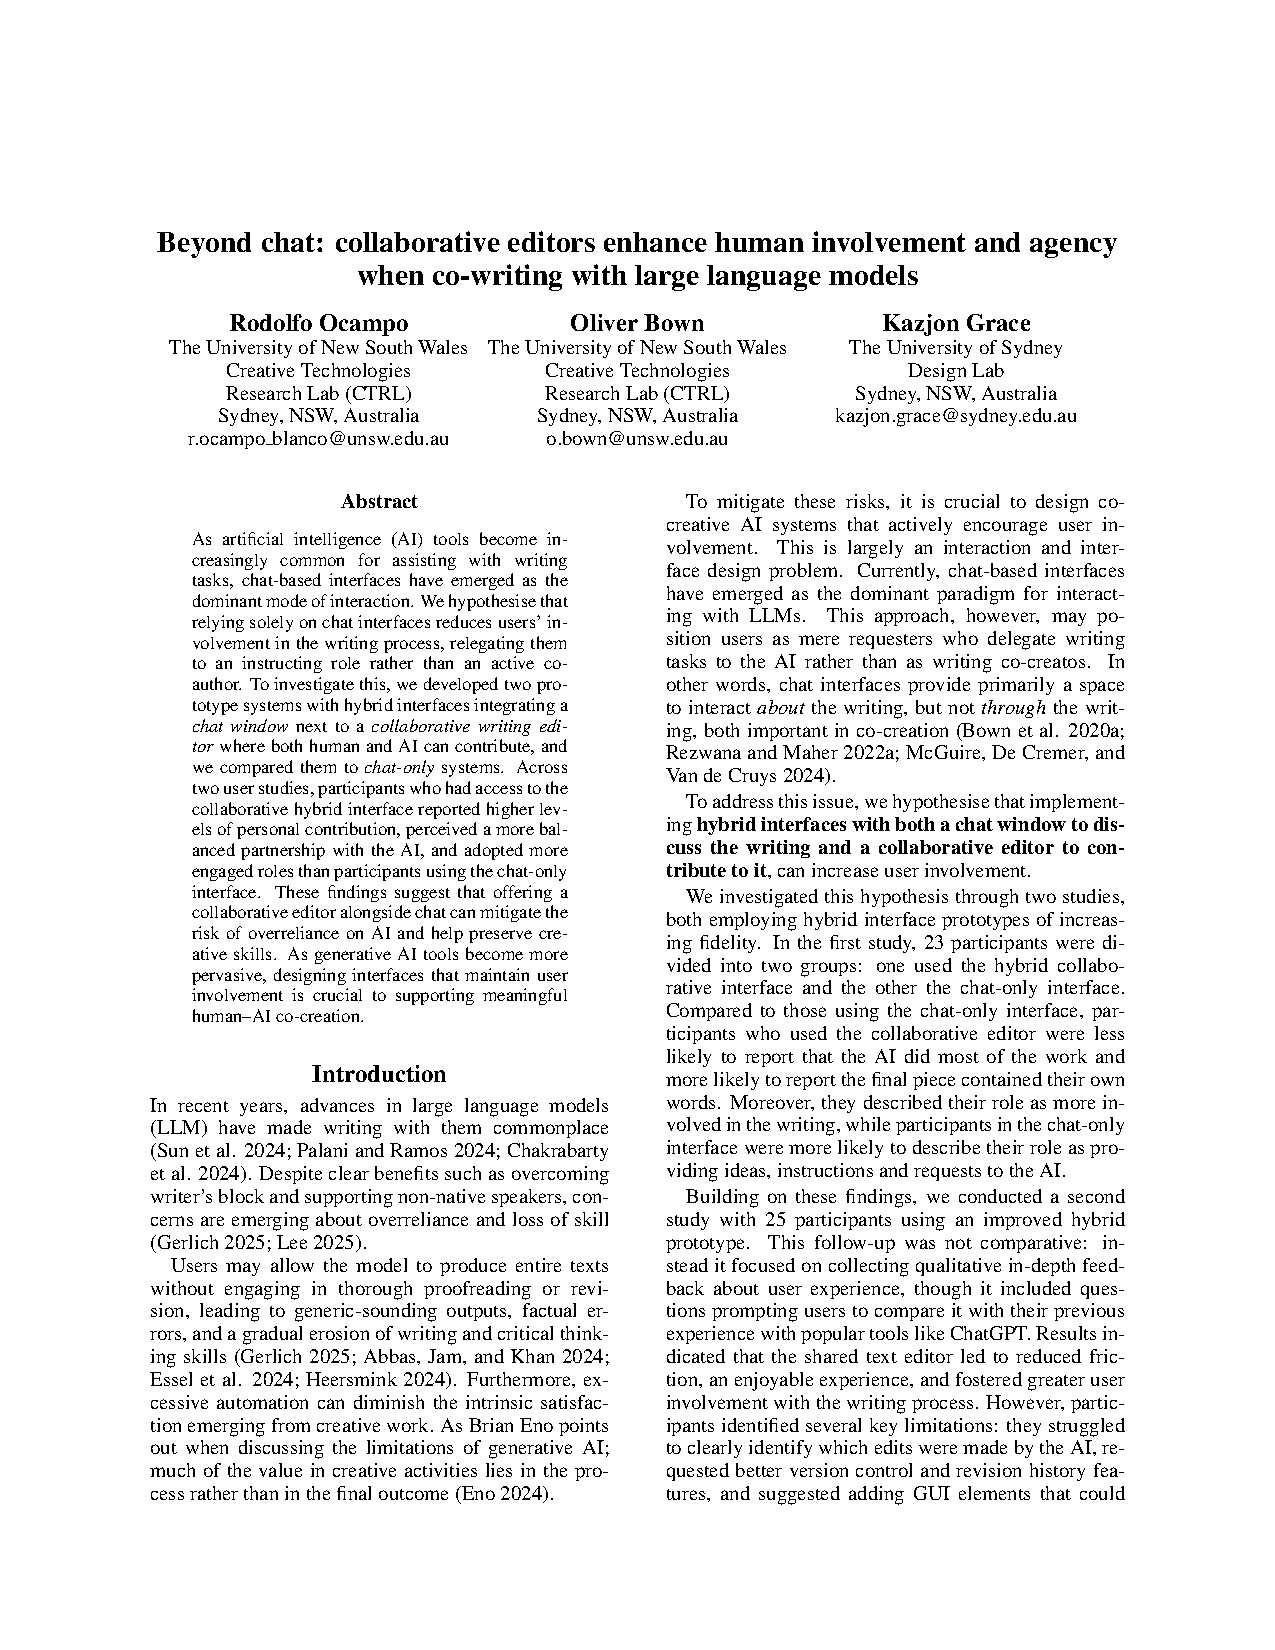
\includepdf[pages=-]{5-Writing/BeyondChat.pdf}
